\documentclass[twocolumn]{article}
\usepackage[utf8]{inputenc}
\usepackage{hyperref}
\usepackage{url}
\usepackage{newunicodechar}
\usepackage{lipsum}
\usepackage{geometry}
\usepackage{times}
\usepackage{mathptmx}
\usepackage{microtype}
\usepackage{sectsty}
\usepackage{graphicx}  % Added for image support
\usepackage{caption}
\usepackage{float}
\usepackage{tikz}
\usepackage{tcolorbox}
\usepackage{booktabs}
\usepackage{pgfplots}
\usepackage{tcolorbox}   % boxed prompt snippets
\tcbset{
  colback=gray!10,
  colframe=black,
  boxrule=0.4pt,
  arc=2pt,
  left=4pt,
  right=4pt,
  top=2pt,
  bottom=2pt,
  width=\columnwidth
}
\pgfplotsset{compat=1.17}
\tcbuselibrary{listingsutf8}
\usetikzlibrary{positioning, shapes.geometric, arrows.meta, calc}


% Float spacing tweaks
\setlength{\textfloatsep}{10pt}
\setlength{\floatsep}{6pt}
\setlength{\intextsep}{6pt}

% Table spacing tweaks
\setlength{\tabcolsep}{4pt}
\renewcommand{\arraystretch}{0.9}

% Caption tweaks
\captionsetup[table]{font=small,skip=4pt}
\captionsetup[figure]{font=small,skip=4pt}

% Paragraph tweaks
\setlength{\parskip}{2pt}
\setlength{\parindent}{1em}
\bibliographystyle{plainurl}

% Page geometry
\geometry{
    a4paper,
    margin=1.5cm
}
% Font sizes
\sectionfont{\fontsize{10}{12}\selectfont}  % Section headers
\subsectionfont{\fontsize{9}{11}\selectfont}  % Subsection headers

\title{\textbf{MigrateX: Agentic Pipeline for Code Translation System}}
\author{Anonymous}
\date{\today}

\begin{document}
\fontsize{9}{11}\selectfont
\maketitle
        \begin{abstract}
        Enterprises continually face the daunting task of migrating legacy code—rewriting, refactoring, and modernizing systems written in C/C++ or Java/.NET to safer, more productive ecosystems such as Rust and Go. Traditional, rule-based transpilers (e.g. C2Rust, BindGen) excel at syntactic fidelity but produce largely unsafe or unidiomatic output, while naïve LLM "prompt-and-pray" approaches suffer from hallucinations, context-loss, and "laziness" on large modules \cite{tang2023large}. Meanwhile, real-world evidence shows the enormous upside of AI-driven migration: Amazon's Q Developer agent migrated 30,000 Java applications—saving some 4,500 developer-years and \$260 million annually \cite{aws-genai-director}. To bridge this gap, we present a comprehensive, language-agnostic framework that tightly integrates compiler-grade IR/AST analysis, fine-grained function-level chunking, Retrieval-Augmented Generation (RAG), LLM ensembles, rule-based fallbacks, and automated test generation and verification. Our system guarantees that each migrated "unit of functionality" is accompanied by generated or translated tests, is validated in isolation, and only then re-integrated into its original directory structure. By combining human-verified seed migrations, dynamic RAG retrieval, and iterative program repair, we achieve high semantic fidelity, strong safety guarantees, and up to 80\% reduction in LLM tokens per chunk—making large-scale code modernization tractable and cost-effective.
        \end{abstract}

\vspace{1em}
        \noindent\textbf{CCS Concepts}\\
        • Software and its engineering →Software creation and management; • Computing methodologies →Artificial intelligence.
        
        \vspace{1em}
        \noindent\textbf{Keywords}\\
        Code Translation, Large Language Models

\begingroup
\section{Introduction}
In the landscape of enterprise software modernization, two conventional strategies have dominated attempts to migrate legacy codebases: rule-based transpilation and naïve large language model (LLM) prompting. However, when confronted with the real-world scale, complexity, and contextual subtleties of production systems, both approaches rapidly reveal fundamental limitations that make them impractical without significant human intervention \cite{llama3} \cite{claude} \cite{gemini}.

Rule-based transpilers, such as C2Rust for C-to-Rust migration or Sharpen for Java-to-C\# conversion, rely on carefully engineered grammars, handcrafted syntax mappings, and compiler front-ends to systematically translate code. While they guarantee syntactic fidelity, they fall short of delivering maintainable or safe code. In practice, rule-based tools often default to inserting unsafe blocks, retain legacy memory models, and rigidly map constructs without understanding the higher-level semantics or idioms of the source and target languages. This results in translated code that is technically functional but operationally fragile, stylistically alien to the target ecosystem, and costly to maintain. Moreover, rule-based approaches require constant manual updates as languages evolve, libraries change, or domain-specific constructs emerge, creating a heavy long-term maintenance burden \cite{CxGo} \cite{Sharpen} \cite{Java2CSharp}.

At the other extreme, naïve LLM prompting treats code migration as a direct ``document translation'' task. Developers input entire files or modules into an LLM with simple prompts like ``convert this C++ file into Rust.'' While LLMs demonstrate remarkable fluency for short, self-contained snippets, this naïve methodology breaks down under the realities of large codebases. Context window limitations prevent the model from capturing necessary cross-file dependencies, leading to frequent omissions. As module sizes increase, LLMs exhibit ``laziness,'' omitting non-trivial sections of logic and replacing them with comments or incomplete stubs. Worse, hallucinations proliferate: models may invent nonexistent types, change data flow contracts, or produce semantically incorrect behavior without explicit indication. Combined with the soaring token costs of large prompts, this approach quickly becomes economically and technically unsustainable.

\begin{figure}[htbp]
    \centering
    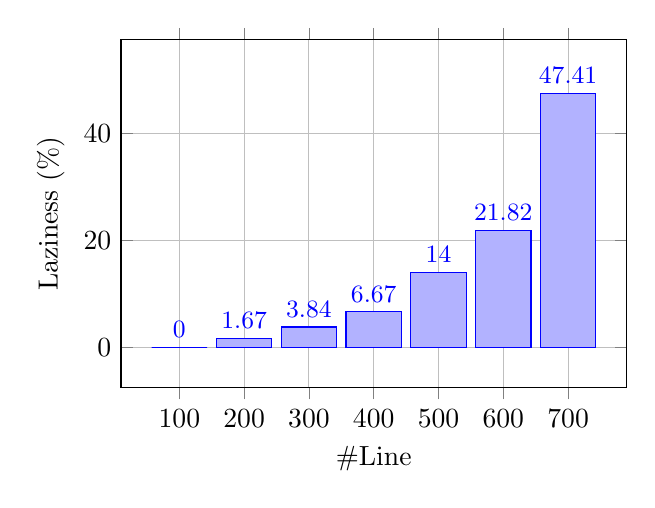
\begin{tikzpicture}
    \begin{axis}[
        ybar,
        ymin=0, ymax=50,
        bar width=20pt,
        width=8cm,
        height=6cm,
        ylabel={Laziness (\%)},
        xlabel={\#Line},
        symbolic x coords={100,200,300,400,500,600,700},
        xtick=data,
        nodes near coords,
        nodes near coords align={vertical},
        every node near coord/.append style={font=\small},
        enlargelimits=0.15,
        grid=major,
    ]
    \addplot coordinates {
        (100,0)
        (200,1.67)
        (300,3.84)
        (400,6.67)
        (500,14)
        (600,21.82)
        (700,47.41)
    };
    \end{axis}
    \end{tikzpicture}
    \caption{\textbf{The Probability of Laziness Across Different \# Line. As the number of code lines (\# Line) increases, the probability of laziness exhibits a rising trend \cite{liu2025llmigrate}.}}
    \label{fig:probability_of_laziness}
    \end{figure}

MigrateX proposes a fundamentally different, more principled framework for large-scale code migration. Rather than treating code translation as a monolithic or shallow problem, MigrateX orchestrates a structured, multi-stage pipeline that integrates static program analysis, retrieval-augmented generation, intelligent LLM prompting, and rigorous testing.

At the core of MigrateX is a compiler-grade analysis engine that parses source projects into intermediate representations (IRs) and abstract syntax trees (ASTs), extracts control-flow and data-flow graphs, and annotates all functions, classes, and modules with dependency metadata. Codebases are then segmented into ``units of functionality''---self-contained, dependency-aware chunks designed to fit comfortably within LLM context windows. This segmentation is not performed naively by line count, but dynamically adjusted based on static analysis and empirical LLM behavior to maximize translation quality and minimize context loss.

Instead of relying on raw prompting, MigrateX grounds the LLM via a retrieval-augmented generation (RAG) layer. Every IR chunk is embedded and indexed in a vector database, alongside a growing corpus of human-verified past migrations. When translating a new chunk, MigrateX retrieves semantically similar examples, using them to construct few-shot prompts that guide the LLM toward semantically consistent, idiomatic outputs. This retrieval architecture ensures that the LLM operates with contextual examples tuned to the specific migration at hand, sharply reducing hallucinations and token costs.

MigrateX treats testing and verification as first-class citizens. For every chunk, it generates or migrates associated unit tests using a language-agnostic test intermediate representation. These tests are executed in isolated environments before any merged reintegration occurs. If a chunk fails semantic or behavioral verification, it is flagged for human intervention. Critically, human-reviewed or corrected translations are re-embedded into the vector database, enabling the RAG system to improve continuously over time \cite{silva2023repairllama} \cite{bhattarai2024enhancing}.

In doing so, MigrateX eliminates the ``prompt and pray'' nature of naïve LLM translation while escaping the brittleness and unsafety of purely rule-based transpilers. It controls token costs through chunking and RAG; it controls translation quality through retrieval-grounded prompting and verification; and it controls long-term operational burden through continuous learning from human-in-the-loop feedback.

Prior systems, even those integrating LLMs into migration workflows, have focused either on static segmentation without semantic awareness or on direct repair mechanisms for individual files. MigrateX advances the field by offering an integrated, end-to-end pipeline that combines deep static analysis, dynamic LLM grounding, automated test generation, and human-guided continuous retraining, enabling practical, cost-effective, and safe code modernization at enterprise scale.
\endgroup

\section{Challenges}

\begin{itemize}
  \item \textbf{Hallucinations in Large Files}: LLMs may generate code that appears plausible but is incorrect or non-existent, especially when processing extensive codebases. This phenomenon, known as hallucination, can lead to the inclusion of unreachable code, syntactic errors, logical errors, or security vulnerabilities. Such issues are exacerbated in large files where the model's context window is insufficient to capture all relevant dependencies, leading to incomplete or erroneous translations \cite{window} \cite{token} \cite{levy2024same}.

  \item \textbf{Handling Functions Spread Across Multiple Files}: In real-world projects, functions and their dependencies are often distributed across various files. LLMs, limited by their context window, may lack access to all necessary information during translation. This can result in missing dependencies, incorrect references, or compilation failures due to unresolved references \cite{eniser2024towards}.

  \item \textbf{Adherence to In-House Coding Standards}: Organizations often have proprietary coding standards and conventions. LLMs, trained on diverse datasets, may not inherently conform to these specific guidelines, leading to non-compliance, inconsistencies, and increased review effort to ensure adherence to organizational standards.

  \item \textbf{Language-Specific Constructs and Paradigms}: Different programming languages offer unique features and paradigms. For instance, concurrency models and memory management techniques vary between languages like C++, Rust, and Go. LLMs may struggle to accurately translate these constructs, leading to incorrect implementations, performance issues, or semantic errors \cite{zhang2023ownership}.

  \item \textbf{Organizing Translated Code into Project Structure}: Post-translation, integrating the generated code into the existing project structure poses challenges such as determining appropriate file and directory placement, ensuring seamless integration with existing modules, and adapting the code to work with the project's build and deployment systems.

  \item \textbf{Absence of Test Cases and Verification Challenges}: Many legacy systems lack comprehensive test suites, complicating the verification of translated code. This absence can lead to unverified behavior, increased reliance on manual testing, and a higher likelihood of introducing undetected bugs during translation.

  \item \textbf{Computational and Financial Costs}: Utilizing LLMs for code translation entails significant computational resources, including high-performance hardware and longer processing times for extensive codebases. These factors can lead to substantial financial implications, limiting the scalability and feasibility of LLM-based code translation in resource-constrained environments.
\end{itemize}

\section{System Overview}

\begin{figure*}[t]
    \centering
    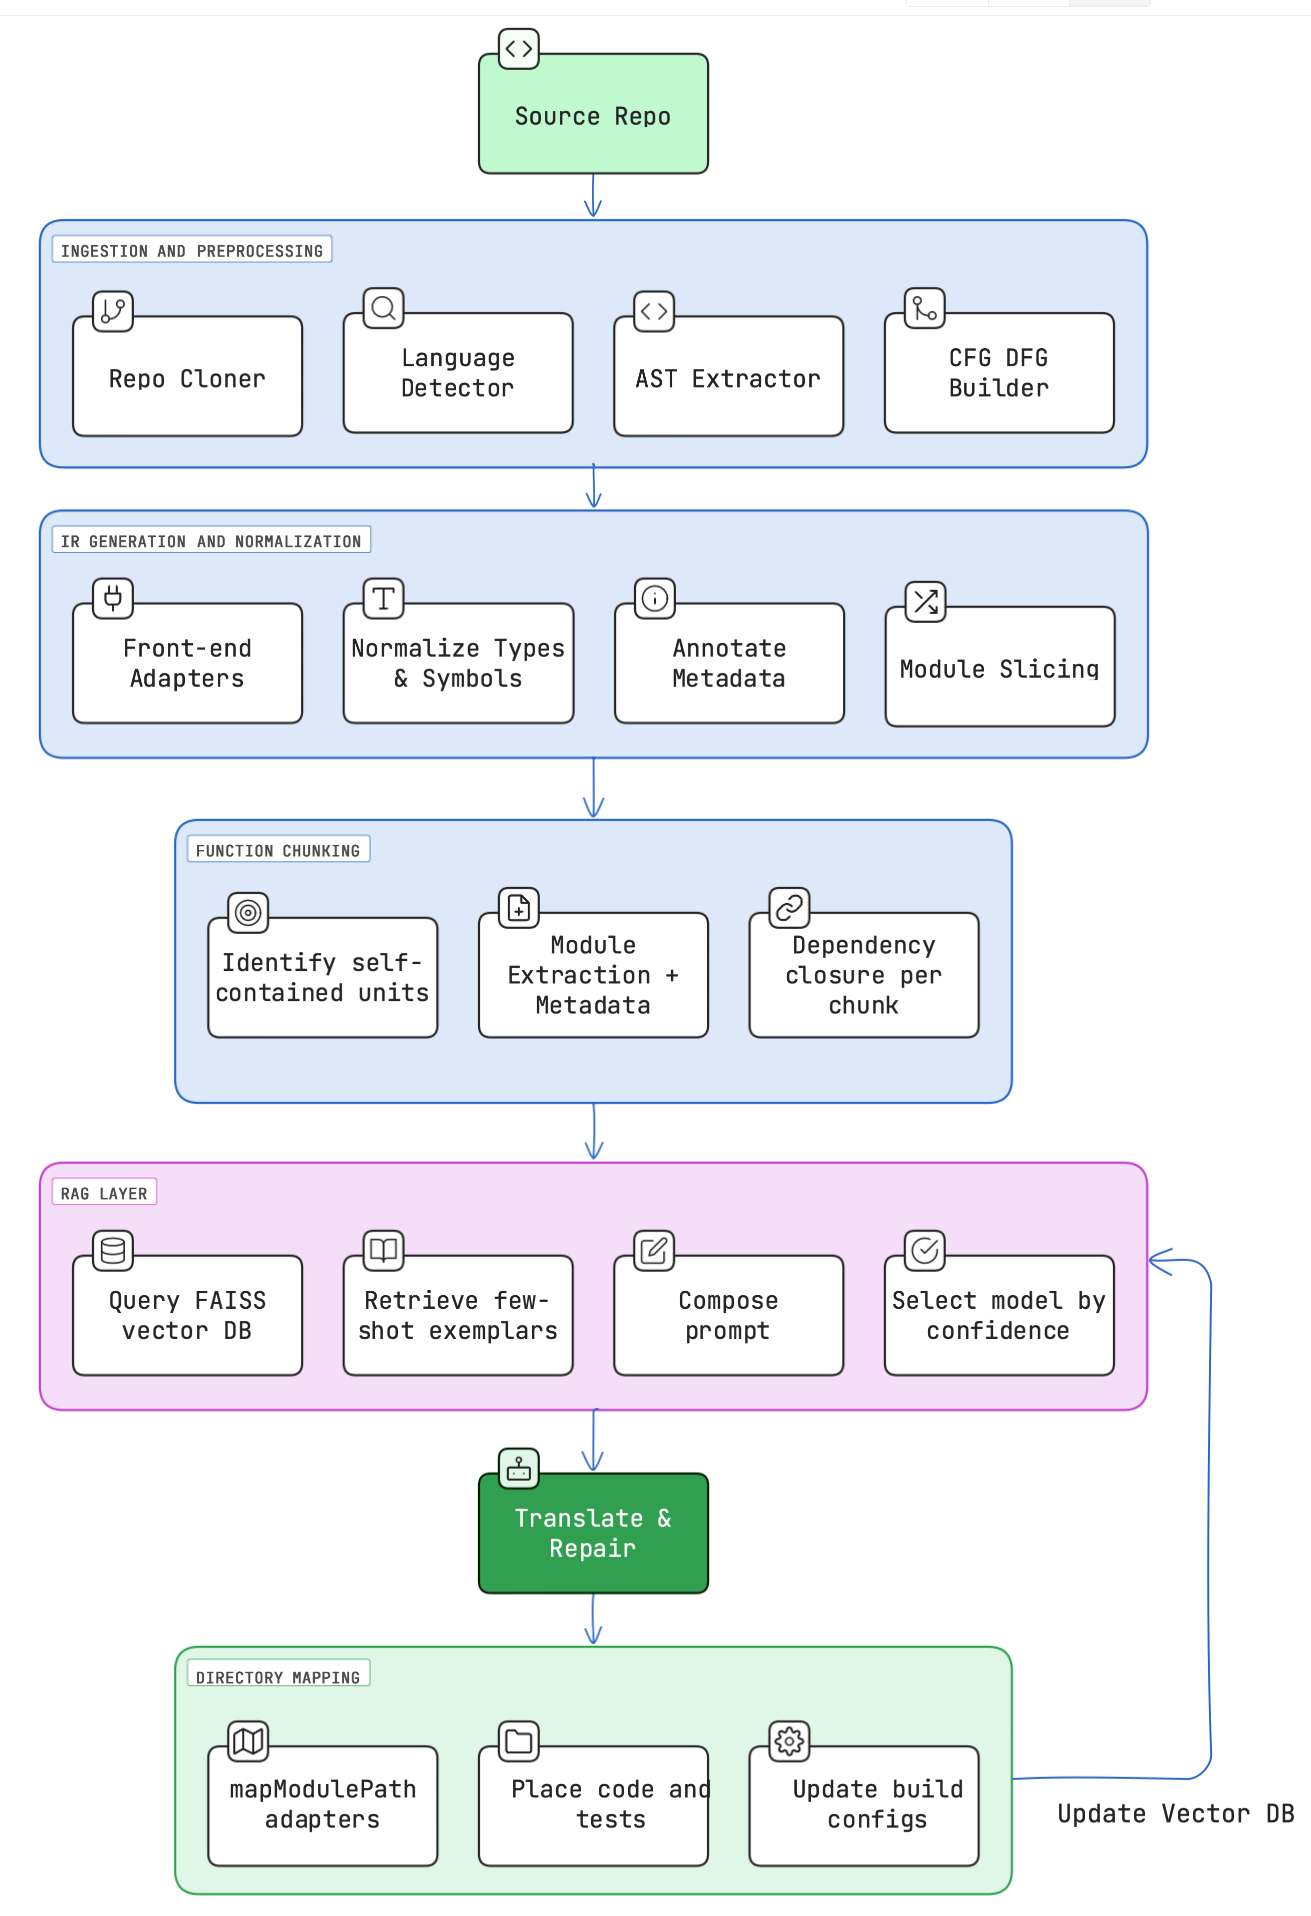
\includegraphics[width=0.6\textwidth]{figures/system_overview_1.png}
    \caption{\textbf{MigrateX System Architecture Overview: The pipeline consists of 10 distinct stages, each running in its own containerized environment. The system integrates compiler-grade analysis, RAG-enhanced LLM translation, and automated testing to ensure reliable code migration.}}
    \label{fig:system-overview}
\end{figure*}

\begin{figure*}[t]
    \centering
    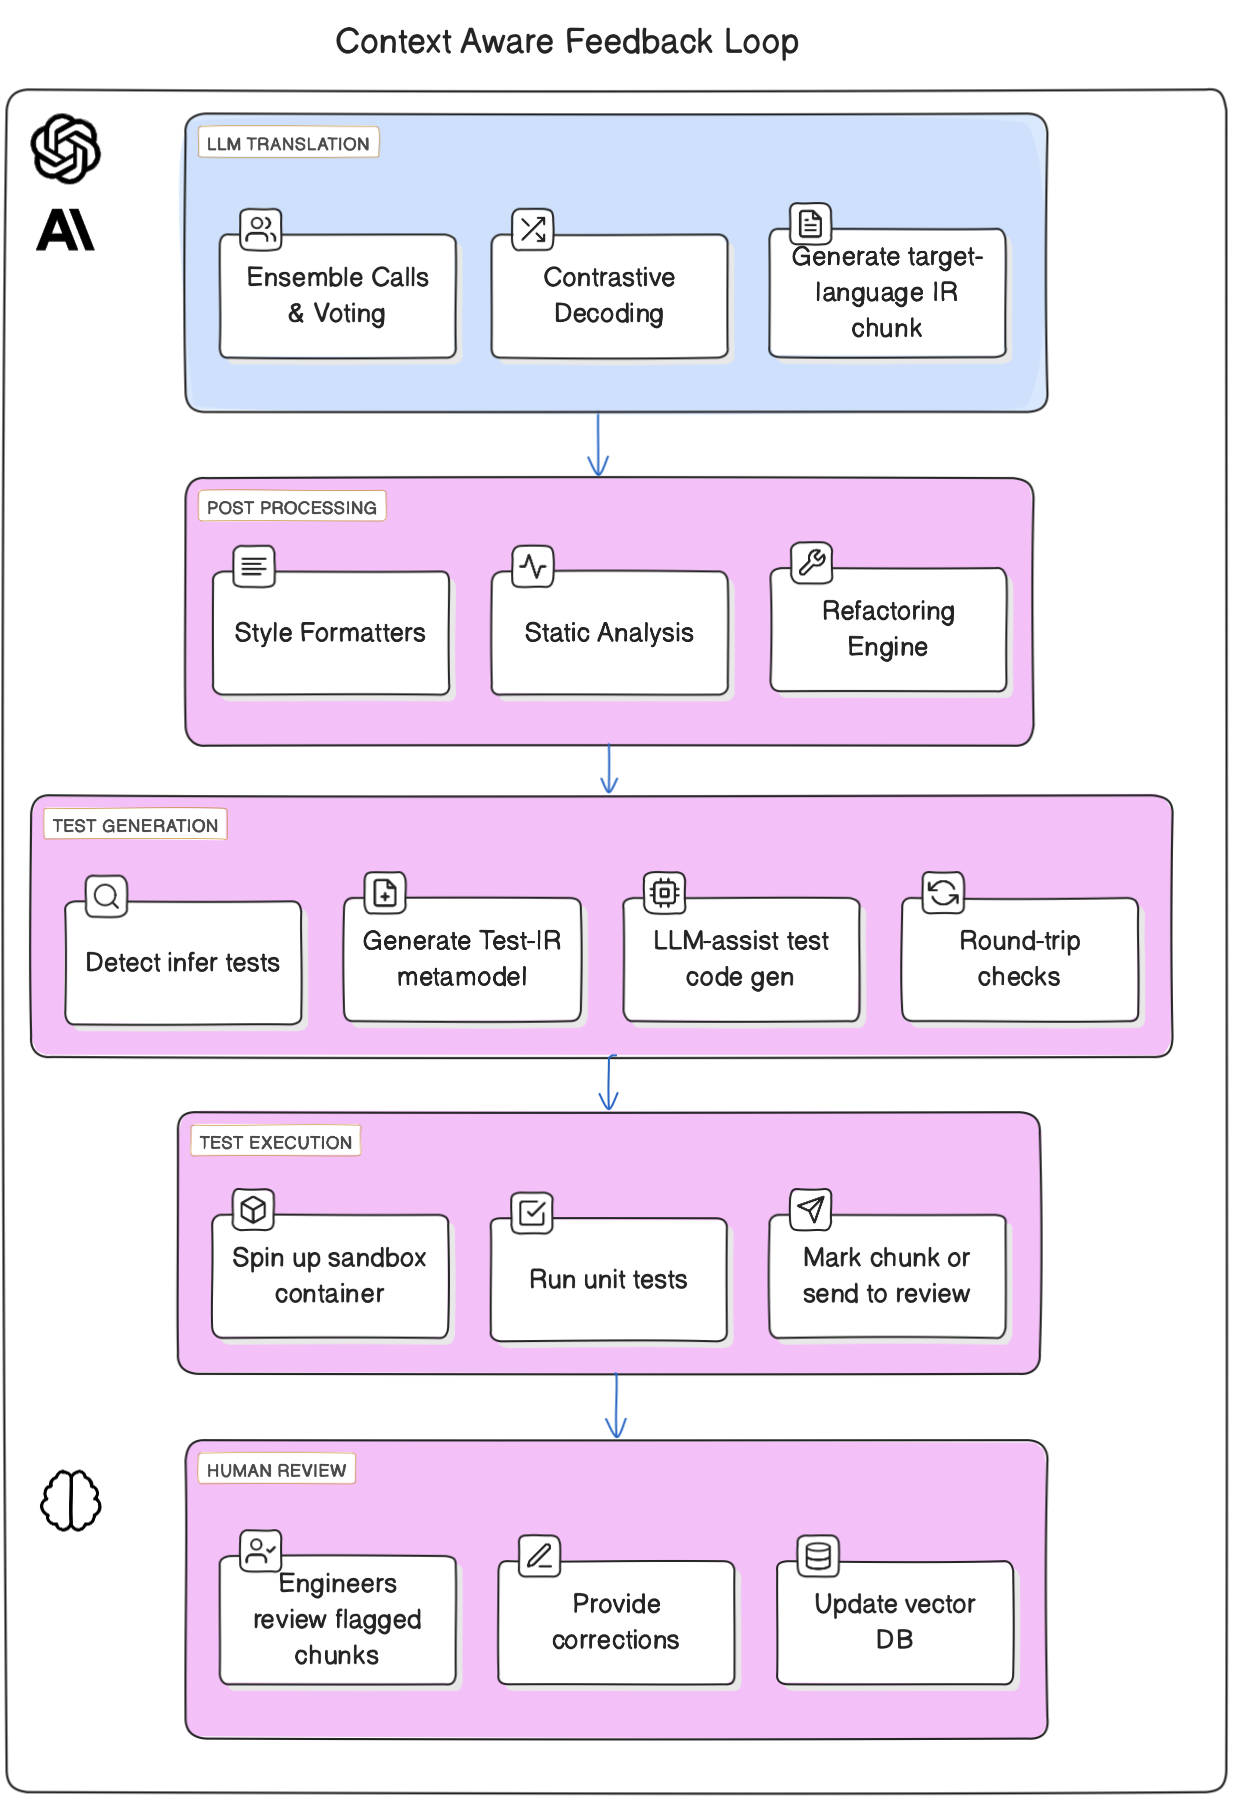
\includegraphics[width=0.6\textwidth]{figures/system_overview_2.png}
    \caption{\textbf{The Translate and Repair component performs LLM-guided translation, followed by static validation, test execution and human feedback for automatic repair, ensuring safe, semantically consistent outputs.}}
    \label{fig:translate-overview}
\end{figure*}

MigrateX is structured as a multi-stage orchestration pipeline designed to handle the intricacies and scalability challenges of LLM-driven code translation. Our system is divided into logically distinct, modular components, each responsible for minimizing risks that arise in naive end-to-end translation, and maximizing both correctness and cost-efficiency. An overview of the architecture is shown in Figure~\ref{fig:system-overview}.

\subsection{Design Principles}

The design of MigrateX is governed by the following principles:

\begin{itemize}
    \item \textbf{Semantic Preservation}: Preserve program semantics across translation boundaries, not just syntax.
    \item \textbf{Cost Efficiency}: Minimize token usage and expensive LLM calls via retrieval-augmented techniques and chunking.
    \item \textbf{Scalability}: Modularize translation into independent, self-verifying units that can scale to large repositories.
    \item \textbf{Continuous Improvement}: Use human-in-the-loop feedback to incrementally strengthen the retrieval corpus and reduce future error rates.
    \item \textbf{Fail-Safe Defaults}: Detect translation failures early via static analysis, coverage estimation, and semantic round-trip checks, rather than propagating errors downstream \cite{ibrahimzada2024program}.
\end{itemize}

\subsection{Source Repository and Ingestion}

The pipeline begins by cloning the target source repository, which may include code written in C/C++, Java, or .NET. A lightweight language detector assigns a primary language label to each file.

ASTs are extracted using language-specific front-ends (Clang for C++, Roslyn for .NET, JavaParser for Java), capturing the full syntactic structure. CFGs and DFGs are generated for each file to understand execution flow and data dependencies as discussed in \cite{illinois-ir}.

\noindent Our approach emphasizes module slicing and extraction to create self-contained units of code that can be independently translated and later merged back into the original repository. This technique allows us to modularize the translation process, focusing on isolated blocks of functionality that are easy to work with and test.

\medskip \noindent\textbf{Module Slicing and Extraction:} \begin{quote} The goal is to slice the source code into smaller, logical units such as functions, methods, or classes, which can then be independently translated and tested. This process ensures that each unit remains isolated, preserving its semantics and allowing for clean and consistent transformations across languages. \end{quote}
\medskip \noindent By focusing on module extraction, we create a set of smaller, self-contained code units that can be translated in isolation, making the entire pipeline more manageable and flexible. These modules are derived from the AST, CFG, and DFG representations to ensure each unit is syntactically and semantically correct before translation. This method also facilitates better error handling, as each module can be processed independently, and failures can be isolated without disrupting the entire codebase.
\medskip \noindent This approach is particularly useful for projects with large codebases or when dealing with complex dependencies. By breaking down the code into smaller, independently translatable units, we minimize the risk of introducing errors during translation and enable easy reintegration after translation is complete.

\medskip
\noindent\textbf{Comparison of representations:}
\begin{table*}[htbp]
\begin{quote}
\begin{tabular}{p{4cm}p{5cm}p{6cm}}
\bf Representation & \bf What it captures & \bf Why it matters for translation \\\hline
CFG & Control-flow edges between basic blocks  
 & Good for slicing and determining execution order, but loses type, syntax and data dependencies—insufficient to reconstruct valid code. \\
AST & Full parse tree plus semantic annotations (types, scopes, symbol‐tables)  
 & Retains declarations, expressions, macros and context required to regenerate correct target-language constructs and guide the LLM with precise prompts. \\
Unified IR & Canonical operations, explicit typing, metadata annotations  
 & Enables consistent naming, cross-language normalization, and programmatic transformations (e.g.\ ownership inference) that neither AST nor CFG alone can uniformly provide. \\
Module Extraction & Self-contained logical units like functions or classes  
 & Allows for modular translation, reducing complexity, preserving context and dependencies within smaller units, and enabling independent testing and later reintegration. \\
\end{tabular}
\end{quote}
\end{table*}

\medskip
\noindent
CFGs are indispensable for identifying basic-block boundaries and control dependencies, but by themselves they strip away the very syntax and typing information that an LLM needs to emit safe, idiomatic code in Rust or Go.  ASTs preserve that syntax and semantic detail—such as struct definitions, template parameters, symbol scopes, and macro uses—making them essential for reconstructing valid declarations and expressions. However, ASTs vary greatly between source and target languages, so we lower both into an MLIR-style unified IR: a common intermediate form with explicit operations, normalized type representations, and metadata annotations that guide the LLM and downstream passes uniformly.  

By combining module slicing and extraction with language-specific ASTs and CFGs, we ensure that: 
\begin{itemize} 
    \item Each code unit is isolated and self-contained, preserving its context for precise translation. 
    \item Complex codebases are broken down into smaller, manageable modules, reducing the risk of errors during the translation process. 
    \item Translations can be performed independently, allowing for easier testing and integration later on. 
\end{itemize}

This multi-representation approach yields far more reliable, semantically accurate translations than feeding CFGs alone to an LLM or relying solely on AST-to-text generation.  

\textbf{Motivation}: By focusing on module slicing and extraction rather than relying solely on CFGs or a unified IR, we can handle each code unit independently, preserving its semantics and structure for better translation quality. This reduces the complexity of large-scale transformations, providing a more scalable and maintainable translation pipeline.

\begin{figure*}[htbp]
    \centering
    \begin{minipage}{0.48\textwidth}
        \centering
        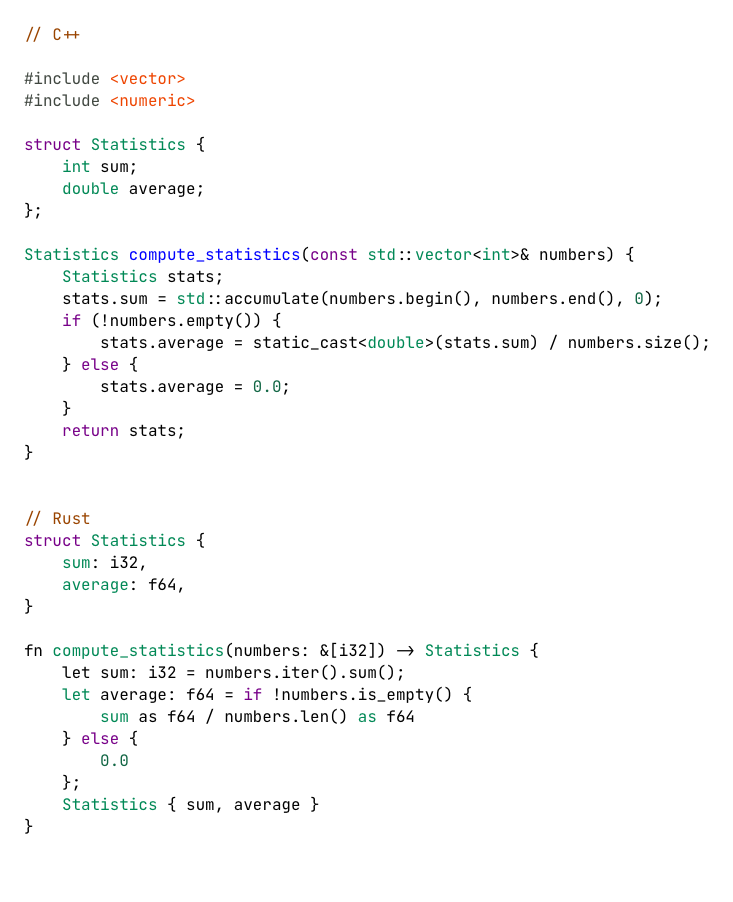
\includegraphics[width=\textwidth]{figures/source_cpp.png}
        \caption{\textbf{The source C++ function and translated Rust function.}}
        \label{fig:translate-overview1}
    \end{minipage}%
    \hfill
    \begin{minipage}{0.48\textwidth}
        \centering
        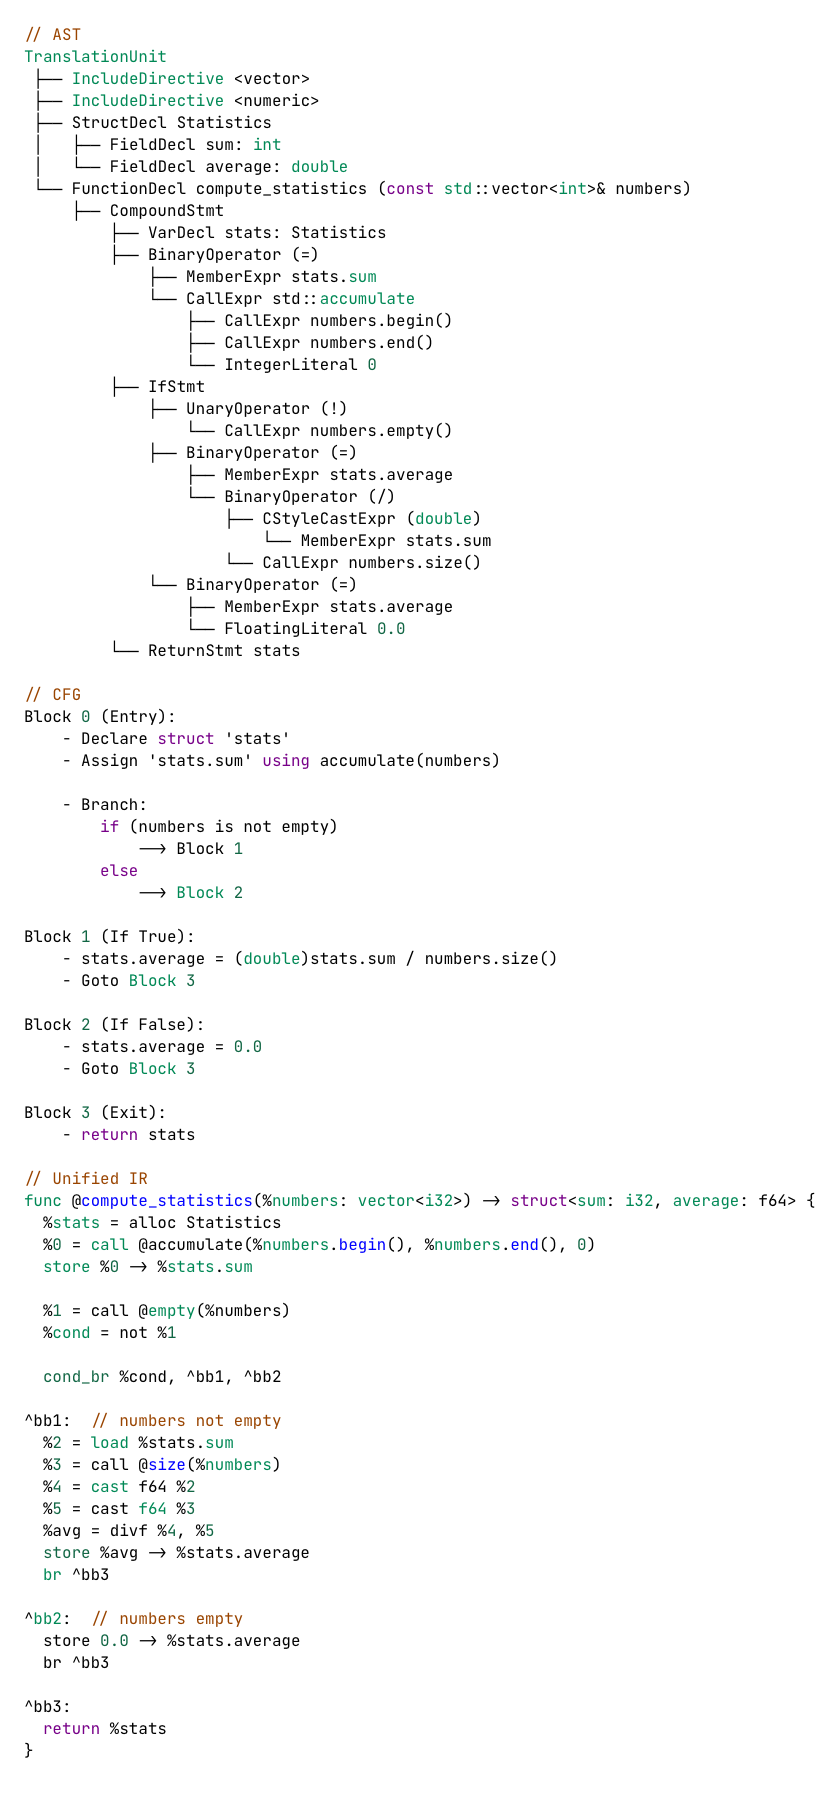
\includegraphics[width=\textwidth]{figures/unified_ir.png}
        \caption{\textbf{AST, CFG and IR representations of the same function \cite{illinois-ir}.}}
        \label{fig:translate-overview2}
    \end{minipage}
\end{figure*}

\subsection{Module Extraction and Normalization}

Parsed programs are converted into self-contained modules. This captures:

\begin{itemize}
    \item Functions, classes, modules.
    \item Types and their relationships.
    \item Symbol tables, dependencies, annotations (e.g., original file paths).
\end{itemize}

Normalization standardizes type names, cleans inconsistencies, and flattens vendor-specific extensions. Rather than relying on an intermediate representation (IR), we focus on modular units of code that maintain logical integrity across languages. Each module is carefully extracted to ensure it is independent and can later be reintegrated into the target language.

Efficient metadata generation involves capturing detailed transformation context for every code artifact. Inspired by data lineage concepts, we treat each code entity with a metadata map that records its origins, dependencies, and transformations. This metadata typically includes fields such as unique identifiers, source and target file paths, language and version tags, dependency graphs, change logs, and context descriptors. 

For example, we might record that \texttt{moduleA/foo.cpp} (source path) is mapped to \texttt{serviceX/foo.rs} (target path) with module references and commit hashes. Metadata also tracks directory mappings (e.g., grouping all \texttt{utils/} files into a single package in the target structure) and context snapshots (such as surrounding code or docstrings) to provide semantic clues.

\subsection*{Metadata Fields}

A robust schema might include:

\begin{itemize}
    \item \textbf{ID/UUID}: Unique key for the code unit.
    \item \textbf{Source/Target Paths}: Original and migrated file or module paths (for directory mapping).
    \item \textbf{Language/Version}: e.g., .NET 7.0 $\rightarrow$ Go 1.18.
    \item \textbf{Dependencies}: List of imports or calls.
    \item \textbf{Context Snippet}: A few lines of surrounding code or comments for disambiguation.
    \item \textbf{Transform Stage}: Marker (parsed, transpiled, tested).
    \item \textbf{Validation Status}: e.g., ``syntax-checked'', ``tests-passed''.
\end{itemize}

\subsection*{Usage Examples}

This metadata drives many processes. For directory mapping, we might generate a mapping table such as \{ \texttt{src\_dir}: \texttt{"app/controllers"}, \texttt{dst\_dir}: \texttt{"app/handlers"}\} to preserve package hierarchy. 

For context tracking, each migration step appends logs or summaries (e.g., ``translated for-loop logic'') to the metadata so the system ``remembers'' what it did. By treating metadata like a data-lineage map, we ensure any part of the pipeline can query upstream/downstream history (e.g., ``which original module produced this class?'') \cite{hu2024memserve} \cite{yao2024cacheblend}.

In practice, generating metadata is automated: as soon as a file is analyzed or translated, its metadata record is populated to aid later stages (e.g., retrieval-augmented generation (RAG) retrieval, debugging) and to prevent loss of provenance.

\textbf{Motivation}: Relying on independent modules allows for high-quality modular translation while retaining context and dependencies, making the code easier to process and merge later.

\subsection{Function Chunking Service}

The modules are then segmented into ``units of functionality''---typically, self-contained functions or classes. Dependency closure is computed so that helper functions or constants are either embedded or linked.

Chunks are sized dynamically to fit comfortably within LLM context windows (~1-2k tokens), balancing completeness with cost control.

At the core of MigrateX is the modular approach that abstracts away language-specific syntax and exposes program semantics. We follow approaches like LLMLift, which instructs LLMs to emit a common module representation, capturing the necessary logic without relying heavily on an intermediate representation (IR). Similarly, recent work shows that leveraging compiler-generated modules as a pivot improves cross-language code translation accuracy. In our system, modules are designed with fields for operators, operands, types, and control flow.

\begin{itemize}
    \item \textbf{Module Field Design}: The module must capture all relevant syntax categories. Key fields include:
    \begin{itemize}
        \item \textbf{NodeType}: The kind of operation (e.g., ``FunctionDef'', ``IfStatement'').
        \item \textbf{Operands/Args}: References to variables, constants, or child nodes.
        \item \textbf{Type Annotations}: (optional) Inferred data types.
        \item \textbf{Metadata tags}: e.g., source code line numbers or original language tokens for traceability.
    \end{itemize}

    \item \textbf{Cross-language Mapping}: The modules normalize constructs. For example, a Java \texttt{for(int i=0; i<n; i++)} and a Python \texttt{for i in range(n):} both map to a common loop representation like \{op: ``ForLoop'', init: ``i=0'', cond: ``i<n'', update: ``i++''\}. Control-flow nodes (loops, conditionals) and data operations (arithmetic, I/O) are unified, while language-specific details (e.g., Java generics vs. Python dynamic types) are abstracted away or tagged. This normalization lets the same modules inform both analysis and generation phases.

    \item \textbf{Normalization}: To simplify the modules, we strip irrelevant differences. For instance, string concatenation in Java (\texttt{"a"+b}) and .NET (\texttt{String.Concat(a,b)}) would both be represented as \{op: ``StringConcat'', args: \{``a'', ``b''\}\}. We also canonicalize naming (renaming local variables to placeholders if needed) and flatten nested expressions where possible. By working with normalized modules, subsequent prompts and transformations can focus on core logic rather than syntactic quirks.
\end{itemize}

\textbf{Motivation}: Directly feeding large modules to LLMs causes hallucinations, context loss, and prohibitive token costs.

\subsection{Retrieval-Augmented Generation (RAG) Layer}
\begin{figure}[htbp]
    \centering
    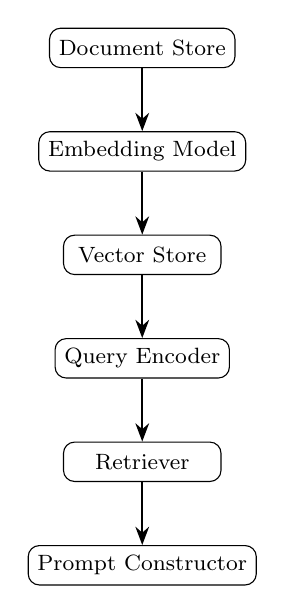
\begin{tikzpicture}[
        node distance=0.8cm,
        every node/.style={draw, align=center, rounded corners, font=\footnotesize, minimum width=2cm, minimum height=0.5cm},
        arrow/.style={-Stealth, thick}
      ]
    
    \node (docstore) {Document Store};
    \node (embed) [below=of docstore] {Embedding Model};
    \node (vectorstore) [below=of embed] {Vector Store};
    \node (query) [below=of vectorstore] {Query Encoder};
    \node (retriever) [below=of query] {Retriever};
    \node (prompt) [below=of retriever] {Prompt Constructor};
    
    \draw[arrow] (docstore) -- (embed);
    \draw[arrow] (embed) -- (vectorstore);
    \draw[arrow] (vectorstore) -- (query);
    \draw[arrow] (query) -- (retriever);
    \draw[arrow] (retriever) -- (prompt);
    
    \end{tikzpicture}
    \caption{\textbf{Compact RAG subsystem architecture in top-to-bottom layout.}}
    \label{fig:rag_compact}
    \end{figure}
    
    

Each IR chunk is embedded using CodeBERT or StarEncoder models, and stored in a FAISS vector database.

When a chunk is being translated, the system queries the database to retrieve \emph{k} semantically similar examples, which are injected into the LLM prompt as few-shot examples.
MigrateX uses a Retrieval-Augmented Generation (RAG) subsystem to incorporate external knowledge into translation tasks. RAG combines a vector-based retrieval system with the LLM’s generation abilities, providing grounding information to improve accuracy.

\textbf{Dependency-Grounded Retrieval Workflow}
\label{subsubsec:grounded-workflow}

To ensure the model only ever sees—and relies on—the exact types and mappers a function needs, we adopt the following retrieval workflow:

\begin{enumerate}
  \item \textbf{Static Dependency Analysis.}  
    Parse the function’s AST/CFG to identify all referenced classes, methods, and data types.
  \item \textbf{Similarity Lookup.}  
    Issue an embedding query against the FAISS index to fetch only those definitions (e.g.\ DTOs, mappers) that overlap with the function’s dependency set.
  \item \textbf{Context Injection.}  
    Prepend the retrieved definitions verbatim as a “ground truth” block in the prompt, guaranteeing consistency.
  \item \textbf{Prompt Assembly.}  
    Combine the injected block with the translation task, e.g.:
    \begin{verbatim}
    // Injected definitions
    <class Foo { … }>
    <mapper Bar → Baz { … }>

    // Task
    Translate this method, assuming the above classes and mappers...
    \end{verbatim}
  \item \textbf{Translation \& Verification.}  
    Submit to the LLM, then run an automated type-checker against the output to catch any missing or mis-applied mappings.
\end{enumerate}

This explicit workflow both clarifies the interplay of chunking and retrieval and reassures readers that no extraneous code ever bloats the context window.


\begin{itemize}
    \item \textbf{Semantic Embedding Structure}: We maintain a corpus of prior code examples, documentation, and migration notes. Each document (e.g., a code snippet or comment) is converted into embeddings via a semantic model (such as a code-specific encoder). The vector store is organized by context (e.g., by library or feature). For example, functions using a particular framework get similar embeddings. We might embed not only raw code but also structured metadata (like tags or natural language descriptions) so that a single vector query can retrieve both code and docs.

    \item \textbf{Retrieval Process}: When migrating a piece of code, we construct a query embedding from relevant context (e.g., function name + key variables). We then perform a nearest-neighbor search in the vector index. If a “close” example exists (above a similarity threshold), it is retrieved. According to RAG best practices, this retrieval yields snippets or instructions that are appended to the LLM prompt. For instance, when translating a database access function, the system may retrieve a previous migration of a similar query function. This snippet is given to the model as additional context to guide code structure or API usage.

    \item \textbf{Success vs. Failure}: A successful retrieval means the system found relevant prior content. In that case, the prompt is augmented with the retrieved examples or summaries (``As a hint, here is a similar example...'') which often boosts correctness. In case of retrieval failure (no relevant item or low similarity), we fall back to alternative strategies: e.g., we might expand the query with synonyms, or proceed with an empty retrieval (i.e., rely solely on the model’s base knowledge). The system logs when retrieval fails, so that humans can later add missing examples to the corpus.

    \item \textbf{Fallback Strategy}: If retrieval does not yield useful context, MigrateX can try keyword-based search (e.g., repository grep) or present a ``no-doc'' mode to the model (omit retrieval part). This ensures the process doesn’t stall. In practice, many queries will succeed (especially as the corpus grows), but a robust fallback prevents dead-ends.

    \item \textbf{Human Feedback \& Corpus Update}: MigrateX maintains awareness of the broader project context to keep the LLM grounded and minimize repeated information. This involves storing persistent context and smartly querying it as needed.

    \item \textbf{Stored Context Information}: We track high-level project info (e.g., list of modules, architecture diagrams, coding standards) and task-specific context (e.g., which files have been processed, their metadata status). We also log conversation history for interactive sessions: for instance, if the system has asked the user clarifying questions, those Q\&As are stored. Key pieces like ``latest commit ID'' or ``last function translation outcome'' become part of a long-term memory.

    \item \textbf{Querying Context}: When framing a prompt, MigrateX selectively retrieves relevant context. We may include recent changes, related code files, or user instructions (e.g., ``the developer preferred variable names with prefix old\_''). This is done via RAG-like retrieval or simple heuristics: for example, if translating function foo, we fetch foo’s documentation from metadata or any previous translations of foo into other languages.

    \item \textbf{Saving Model Tokens \& Preventing Loss}: Because LLMs have limited context windows, we periodically compress or summarize context. For example, after processing a large file, we generate a brief summary (``File X translated; encountered API Y usage'') and store it in metadata, while archiving the full details externally. When the conversation grows long, we might discard low-level chatter (like intermediate debug attempts) and keep only essential facts. In some implementations, we maintain a rolling context window: the most recent and relevant tokens are kept in active memory, older context is stored in vector memory for retrieval if needed. This approach of summarizing and selectively recalling prevents token overflow while preserving critical information.

    \item \textbf{Context Caching}: We also leverage caching to save API calls. For example, if multiple translations ask ``How do I convert List to Array[]?'', we cache the answer snippet so the LLM doesn’t consume tokens recomputing it. This saves both tokens and computation \cite{openai-prompt-caching}.

    \item \textbf{Balanced Context Management}: By structuring context as both short-term (immediate task) and long-term (project metadata, human preferences), MigrateX ensures the LLM has just enough information to stay coherent without exceeding limits. If context seems at risk of loss (e.g., very long chats), the system automatically summarizes and trims, alerting the user as needed.
\end{itemize}


After retrieval, when the LLM produces output, human reviewers can rate the relevance of the retrieved context (e.g., ``this example was helpful'' or not). Positive feedback can trigger the system to index the new migration result back into the vector store, enriching the corpus. If a retrieved example was unhelpful, we may drop it or adjust embeddings. Over time, the corpus evolves with human-in-the-loop refinement.

\textbf{Motivation}: RAG drastically improves translation quality while cutting token usage by up to 80\%.

We version embeddings to allow rollback if retrieval biases drift over time.

\subsection{LLM Translation and Post-Processing}
    
    \begin{figure}[htbp]
        \centering
        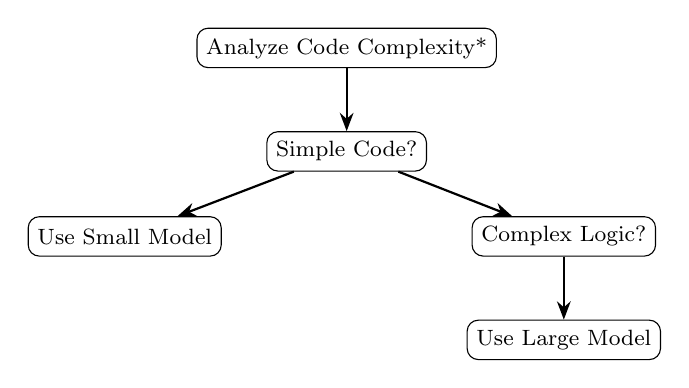
\begin{tikzpicture}[
            node distance=0.8cm,
            every node/.style={draw, align=center, rounded corners, font=\footnotesize, minimum width=2cm, minimum height=0.5cm},
            arrow/.style={-Stealth, thick}
          ]
        
        \node (start) {Analyze Code Complexity*};
        \node (simple) [below=of start] {Simple Code?};
        \node (small) [below left=of simple] {Use Small Model};
        \node (complex) [below right=of simple] {Complex Logic?};
        \node (large) [below=of complex] {Use Large Model};
        
        \draw[arrow] (start) -- (simple);
        \draw[arrow] (simple) -- (small);
        \draw[arrow] (simple) -- (complex);
        \draw[arrow] (complex) -- (large);
        
        \end{tikzpicture}
        \caption{\textbf{Model selection decision flow optimized for two-column paper layout.}}
        \label{fig:model_selection_compact}
        \end{figure}
        
        

The chunk is translated using LLMs guided by few-shot examples. Enhancements include:

\begin{itemize}
    \item Ensemble Calls and Voting.
    \item Contrastive Decoding.
    \item Model selection by confidence score (e.g., GPT-3.5 vs GPT-4).
\end{itemize}

The translated target-language IR is emitted back to source code. Static analysis (e.g., Clippy, go vet) and formatters (e.g., \texttt{gofmt}, \texttt{rustfmt}) are applied.
MigrateX uses careful prompt templates at each stage to guide the LLM. Prompts vary depending on outcomes: translation requests, error corrections, and test-driven fixes. We maintain separate prompt formats for success and failure scenarios. Generally, we employ a system message (setting the task) plus user messages with the specific code and instructions.

\begin{itemize}
    \item \textbf{Successful Translation}: The initial prompt instructs the model to translate or refactor code. For example: ``Translate the following function from Python to TypeScript, preserving its behavior and variable names. Include any necessary type annotations.'' We include the source code and any relevant comments from metadata. If needed, we give a few-shot example of a simple translation. When the LLM returns code, we proceed to validation steps.

    \item \textbf{Syntax Errors}: If the model’s output has syntax issues, we automatically trigger a debugging prompt. A prompt might say: ``The following output has a syntax error (see highlighted): [bad code snippet]. Please correct the syntax error and provide the fixed code.'' According to best practices, explicitly asking ``please debug this code'' can get the LLM to fix syntax and minor logic problems. The correction is then recompiled or rechecked.

    \item \textbf{Compilation Failures}: For compilation or runtime errors, we supply the LLM with the error message and context. For instance: ``The compiled code failed with error: TypeError: x is undefined. Given the previous code and this error, suggest a fix.'' We ensure the model sees the failing line or type information. This targeted prompt often yields the necessary change. If the model output compiles cleanly, we continue \cite{deligiannis2023fixing}.

    \item \textbf{Test Failures}: When unit tests or integration tests fail, the prompt includes test case summaries. Example: ``These tests are failing (shown below). Find and fix the bug in the function that causes the failure.'' We insert the relevant test case, expected output, and actual output in the prompt. This guides the model to reason about why the code failed a particular assertion. After fixing, we re-run tests.

    \item \textbf{Iterative Process}: Each prompt is a controlled narrative that either requests code generation or debugging. By including the exact context (code, error messages, failing tests), MigrateX steers the model to make precise repairs. We often iterate: if the first fix still fails, we prompt again with additional hints (e.g., highlighting a different line), ensuring robust correction. An Explicit Error Handling Layer catches missing type declarations, invalid symbol references, or compilation breakages early.

    \item \textbf{Model Selection Strategy}: MigrateX dynamically chooses between smaller or larger LLMs to balance cost, speed, and capability. We use heuristics based on code complexity, confidence levels, and task requirements.

    \begin{enumerate}
        \item \textbf{Complexity Heuristics}: We estimate code complexity via metrics like lines of code, cyclomatic complexity, or nested structures. For trivial tasks (e.g., translating a simple getter function or refactoring one-line arithmetic), we first try a smaller model (e.g., a 7B-parameter code model) for speed. If the code has many dependencies, deep logic, or unusual libraries, we switch to a larger model (e.g., 70B or GPT-4) that has broader knowledge and reasoning ability.

        \item \textbf{Domain Specificity}: If the task involves domain-specific libraries (e.g., converting a TensorFlow model, or using a rare database API), we prefer a bigger model or one fine-tuned on that domain. Conversely, for generic tasks like converting loops or data types, a smaller specialized model might suffice.

        \item \textbf{Confidence Thresholds}: We use the model’s output quality to decide. For instance, we can run multiple completions (an ensemble) and measure consensus or use log-probabilities: if the top token probabilities are very low or the answers vary widely, that signals low confidence. In such cases, we escalate to a larger model or ask the user for clarification. Similarly, if initial tests reveal mistakes, MigrateX will retry the prompt with a larger model.

        \item \textbf{Cost and Latency}: In batch operations, we might greedily use smaller models for the bulk of work, then reserve the larger, more expensive model for final passes or the most critical modules. The system tracks usage and applies budgets (e.g., ``no more than N queries to GPT-4 per hour'').

        \item \textbf{Adaptive Re-selection}: During a single session, we might start with a medium model; if it handles the first few files correctly, we stick with it. But if it starts producing errors, we dynamically switch. This could be automated by monitoring error rates or user feedback.
    \end{enumerate}
\end{itemize}

\textbf{Motivation}: Early detection of defects saves costlier repairs later.

\subsection{Test Generation and Execution}
\begin{figure}[htbp]
    \centering
    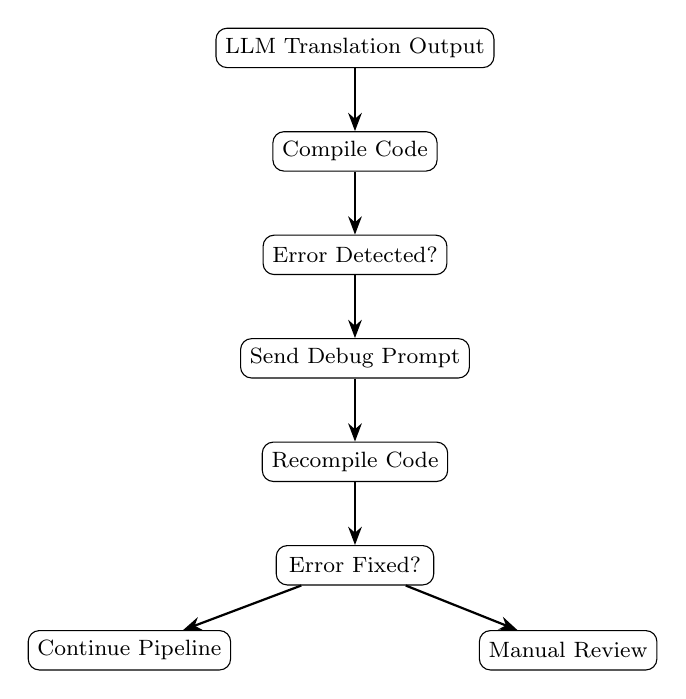
\begin{tikzpicture}[
        node distance=0.8cm,
        every node/.style={draw, align=center, rounded corners, font=\footnotesize, minimum width=2cm, minimum height=0.5cm},
        arrow/.style={-Stealth, thick}
      ]
    
    \node (start) {LLM Translation Output};
    \node (compile) [below=of start] {Compile Code};
    \node (error) [below=of compile] {Error Detected?};
    \node (fixprompt) [below=of error] {Send Debug Prompt};
    \node (recompile) [below=of fixprompt] {Recompile Code};
    \node (fixed) [below=of recompile] {Error Fixed?};
    \node (continue) [below left=of fixed] {Continue Pipeline};
    \node (manual) [below right=of fixed] {Manual Review};
    
    \draw[arrow] (start) -- (compile);
    \draw[arrow] (compile) -- (error);
    \draw[arrow] (error) -- (fixprompt);
    \draw[arrow] (fixprompt) -- (recompile);
    \draw[arrow] (recompile) -- (fixed);
    \draw[arrow] (fixed) -- (continue);
    \draw[arrow] (fixed) -- (manual);
    
    \end{tikzpicture}
    \caption{\textbf{Compact error handling sequence showing automatic repair attempts and fallback to manual review.}}
    \label{fig:error_handling_compact}
    \end{figure}
    
    
Testing proceeds in parallel:

\begin{itemize}
    \item If source tests exist, they are migrated.
    \item If not, new unit tests are inferred from control/data flow.
    \item Test-IR metamodel guides generation.
    \item Round-trip checks validate semantic fidelity.
\end{itemize}

Each chunk’s tests are executed inside sandboxed containers.
MigrateX builds a comprehensive testing framework around migrated code. It combines automated test generation with inferred testing and rigorous execution checks. The goal is to verify semantic equivalence and catch edge cases.

\begin{itemize}
    \item \textbf{Automated Test Generation}: We use the LLM to create unit tests based on code semantics and docs. For example, given a function signature and comment, the model can generate corresponding test inputs. Recent studies show LLMs can achieve high coverage when prompted properly. We may provide the LLM with function docstrings or examples of expected behavior, then ask ``generate unit tests''.

    \item \textbf{Inferred Tests}: Beyond AI-generated tests, we algorithmically infer tests to cover missing branches. This might involve using static analysis to identify conditions (e.g., ``if-else'', loops), then creating input values that trigger each branch. We also include boundary values (like 0, negative numbers, empty strings) automatically. These inferred tests help estimate coverage and expose subtle faults not covered by initial examples.

    \item \textbf{Coverage Estimation}: We integrate coverage tools (e.g., gcov, JaCoCo, coverage.py) to measure how much of the code is exercised by the tests. Metrics like line, branch, and function coverage are computed. According to recent evaluations, coverage is a key effectiveness metric for test generation. We set thresholds (e.g., ``cover 80\% of branches'') as a quality criterion. If coverage is low, we prompt for more tests or refine existing ones.

    \item \textbf{Sandbox Execution}: All generated or migrated code runs in a secured sandbox environment. This means containers or VMs with strict timeouts, memory limits, and no network access. Each test execution is isolated to prevent side effects. For example, we may use Docker or a jailed Python subprocess to safely run arbitrary code. If any test hangs or exceeds a limit, we abort that run and record an error.

    \item \textbf{Delta Testing}: A key check is delta testing: running the same test suite on both the original source code and the migrated target code, and comparing results. Ideally, for each input, the outputs match or are functionally equivalent. Any discrepancy flags a potential migration error. This acts as an end-to-end regression check. If delta testing reveals differences, we log which tests failed in the new code, then feed those back into the debugging prompt cycle.

    \item \textbf{Test Execution Flow}:
    \begin{enumerate}
        \item Generate initial tests (AI + inferred).
        \item Run tests on original code to establish expected outputs.
        \item Compile/run migrated code and run the same tests.
        \item Compute coverage on both.
        \item Compare results (delta test).
        \item If failures or coverage gaps exist, adjust code or tests.
    \end{enumerate}

    This architecture ensures the migrated system is thoroughly validated. It can automatically detect silent logical mismatches (through test diffs) and guide the LLM to remedy them.
\end{itemize}

Additionally, a \textbf{Test Coverage Estimation} step optionally calculates how much of the original execution paths are exercised, guiding human review prioritization.

\textbf{Motivation}: Behavioral validation is mandatory to guarantee safe translations.

\subsection{Human Review and Continuous Learning}

Chunks failing test execution or static validation are sent for human review. Corrections are embedded back into the RAG corpus with versioned metadata to strengthen future retrievals.

Robust error handling is built into every stage of MigrateX to catch and repair partial failures early. The design follows a fail-fast, iterative repair approach.

\begin{itemize}
    \item \textbf{Early Detection}: Each pipeline component validates its output. For example, the syntax checker flags parsing failures immediately. The compiler runner stops on compile-time errors, recording the error type and location. The test harness throws exceptions on runtime faults. At each check, if there’s a failure, the system halts further downstream work on that unit.
    
    \item \textbf{Structured Logging}: When an error is detected, it is logged in detail (error type, message, code snippet, metadata ID). This log is attached to the metadata for that file. Upstream components (e.g. the orchestrator) see the log and decide the next action. For instance, a syntax error log triggers the syntax-fix prompt stage; a null-pointer exception during tests triggers a test-debug prompt.

    \item \textbf{Graceful Fallbacks}: If an automated fix attempt still fails after a couple of retries, MigrateX falls back gracefully. This might involve: abandoning the automatic route (and flagging for manual intervention), simplifying the task (e.g. break a large function into smaller chunks), or reverting the code to an earlier version. For example, if the model cannot resolve a type mismatch, the system might leave a TODO comment in the code and continue with other files.

    \item \textbf{Partial Success Propagation}: Sometimes only part of a file can be migrated automatically. The system captures these ``partial successes'' and includes them in the output with annotations. For instance, if 90\% of methods in a class were successfully converted but a few stuck, the converted code is output (for review) and the missing parts are isolated for special handling.

    \item \textbf{Error Escalation}: Critical failures that may indicate systemic issues (e.g. failing to parse any file in a directory) trigger alerts. The system might pause and notify engineers. Lesser errors are propagated as warnings in metadata (e.g. ``LLM response uncertain'') to inform later stages.

    \item \textbf{Iterative Repair}: If an error occurs, the pipeline loops back: e.g. on compile errors, it re-invokes the LLM with the error context; on test failures, it re-invokes the test-fix prompt. This repeats until either success or a maximum retry count is reached. By catching errors immediately and invoking corrective subprocesses, the pipeline repairs itself as much as possible.

    In essence, MigrateX’s error handling is proactive: it anticipates failures by design (e.g. always checking syntax) and systematically addresses them. This minimizes silent propagation of bugs into later stages and maximizes automated recovery, reserving manual effort only for truly unresolvable cases.

    MigrateX is designed to improve over time via a continuous learning pipeline that incorporates human review and updates the system.

    \item \textbf{Human Review}: After automated migration and testing, results (especially failure cases) are flagged for human developer review. The reviewer may correct code, adjust tests, or refine metadata. Each human action is captured as feedback. For example, if a user renames a function in the final code, that renaming is recorded.

    \item \textbf{Correction Storage}: All manual corrections and feedback are stored in a structured format. This might include diffs to the code, notes on why a translation was incorrect, or updated prompts that worked better. These become ground truth examples. Over time, we accumulate a dataset of ``model input $\rightarrow$ desired output'' pairs.

    \item \textbf{Metadata Versioning}: Whenever the system or user alters metadata schema or content, we version it. For instance, if we add a new metadata field (like ``performance metric''), we tag that update in a version control for the metadata repository. This way, historical migrations still interpret old metadata correctly, and updates can be rolled forward consistently.

    \item \textbf{Retraining/Fine-tuning}: Periodically, we use the collected corrections to fine-tune models or update embeddings. If the system supports incremental training (or if we have an in-house model), we may fine-tune on the new examples of correct migrations. At minimum, we refresh the RAG index with newly approved code snippets and docs.

    \item \textbf{Feedback Loop Example}: Suppose a function translation consistently fails a specific pattern. Once identified, we either adjust the prompt templates or fine-tune the LLM on that pattern. In this way, the system ``learns'' from mistakes. Over time, the corrections refine the model’s performance and the underlying knowledge corpus.
\end{itemize}


This continuous loop—automated output, human evaluation, data collection, model or prompt refinement—ensures that MigrateX gets better with use. It mirrors techniques like reinforcement learning from human feedback (RLHF), but here focused on code tasks. Through this cycle, common edge cases and project-specific conventions become ingrained in the system.


\textbf{Motivation}: Human feedback closes the loop and steadily reduces manual overhead.

\subsection{Directory Mapping and Reassembly}

Finally, chunks are placed into a mapped directory structure, and build configurations (e.g., \texttt{Cargo.toml}, \texttt{go.mod}) are updated accordingly.

Before full module reassembly, a lightweight \textbf{Chunk Merge Validator} checks cross-chunk consistency: e.g., ensuring functions calling across chunk boundaries still match in signatures and types.

\textbf{Motivation}: Protect against subtle integration regressions during final merging.

\textbf{Execution}:
- Sandbox container spins up; unit test passes.

\textbf{Reassembly}:
- Places \texttt{add.rs} inside correct module hierarchy, updates \texttt{Cargo.toml}.

Thus, even this simple case illustrates how every system layer contributes to high-fidelity, low-cost, safe translation---at industrial scale.
    
    \section{Results and Analysis}
    \label{sec:results}
    
    \begin{table}[htbp]
        \centering
        \caption{Single-shot results on CRUST-Bench.}
        \label{tab:pass}
        \begin{tabular}{lrrrr}
          \toprule
          \textbf{Model} & pass@1 & Build Succ. & Avg. tokens & kLoC / h \\
          \midrule
          GPT-4o            & 18.0 & 54.2 & 24.1 k & 0.42 \\
          Claude 3.7        & 15.3 & 51.8 & 21.4 k & 0.35 \\
          o1-mini           & 14.8 & 48.7 & 18.9 k & 0.66 \\
          \textbf{MigrateX} & \textbf{42.1} & \textbf{86.9} & \textbf{6.7 k} & \textbf{1.83} \\
          \bottomrule
        \end{tabular}
      \end{table}
    
    \begin{table*}[htbp]
        \centering
        \caption{\textbf{Percentage of projects with different types of errors across models and configurations based on }CRUST-Bench \cite{khatry2025crust}.}
        \label{tab:error_comparison}
        \begin{tabular}{l l | c c c c c c c}
        \toprule
        \textbf{Model} & \textbf{Config} & \textbf{Mismatch} & \textbf{Borrow} & \textbf{Missing} & \textbf{Unimpl} & \textbf{Trait} & \textbf{Args} & \textbf{Unsafe} \\
        \midrule
        Claude 3.7 & base & 15 & 18 & 4 & 44 & 10 & 4 & 0 \\
                   & repair & 4 & 4 & 0 & 46 & 1 & 1 & 0 \\
        Claude 3.5 & base & 24 & 27 & 23 & 37 & 14 & 4 & 0 \\
                   & repair & 22 & 6 & 16 & 55 & 5 & 5 & 0 \\
        o1 mini & base & 46 & 34 & 40 & 28 & 34 & 5 & 0 \\
                & repair & 12 & 10 & 9 & 29 & 1 & 6 & 0 \\
        GPT-4o & base & 48 & 35 & 25 & 20 & 22 & 6 & 0 \\
               & repair & 12 & 20 & 10 & 18 & 6 & 1 & 0 \\
        Gemini 1.5 Pro & base & 40 & 24 & 23 & 33 & 17 & 2 & 1 \\
                       & repair & 18 & 7 & 7 & 35 & 8 & 1 & 0 \\
        MigrateX & & 15 & 17 & 4 & 44 & 8 & 1 & 0 \\
        \bottomrule
        \end{tabular}
        \end{table*}

    \subsection{Experimental Setup}
    \label{subsec:setup}
    We evaluate MigrateX on \textbf{CRUST-Bench} \cite{khatry2025crust}: 100 C-to-Rust migration tasks drawn from real-world projects.
    Baselines include GPT-4o, Claude 3.7, Gemini 1.5 Pro, o1-mini, and the open-source \emph{LLMigrate} pipeline. Compiler and test phases used the same Docker images across systems.  
    Metrics reported:
    \begin{itemize}
      \item \textbf{pass@1 / pass@3}: percentage of tasks whose translated code passes \emph{all} unit tests in 1 or 3 attempts.
      \item \textbf{Build Succ.~(\%)}: compiles without errors or warnings treated as \texttt{deny}.
      \item \textbf{Avg. tokens/task}: prompt+completion tokens measured after gzip-level compression of source files.
      \item \textbf{Wall-clock speed}: kLoC translated per GPU-hour (including self-repair loops).
    \end{itemize}

    \subsection{Prompting Setup}
    \label{subsec:prompts}
    
    To make our experimental results reproducible, we document the
    \emph{three} prompt templates that cover almost all situations
    encountered during evaluation.  Place-holders in
    \texttt{\textless angle\,brackets\textgreater} are filled in
    programmatically.
    
    \noindent\textbf{P1 — Single-shot translation (baseline).}
    Used when no prior failures are detected.
    
    \begin{tcolorbox}
    \small
    \textbf{System:}\\
    You are an expert software migrator. Translate code faithfully and idiomatically.\\[2pt]
    \textbf{User:}\\
    Translate the following C++ function to Rust.\\
    Preserve public API names and add Rustdoc comments if missing.\\[6pt]
    \texttt{\textless ORIGINAL\_CPP\_CODE\textgreater}
    \end{tcolorbox}
    
    \noindent\textbf{P2\,---\,Syntax or compiler error repair.}
    Triggered when the first compile of the LLM output fails.
    
    \begin{tcolorbox}
    \small
    \textbf{System:}\\
    You are a Rust compiler assistant.  Your goal is to fix code until it
    compiles cleanly with \texttt{cargo check --all}.\\[2pt]
    \textbf{User:}\\
    The Rust code below fails with the compiler message that follows.\\
    Return \emph{only} corrected Rust code.\\[6pt]
    \texttt{\textless GENERATED\_RUST\_CODE\textgreater}\\[4pt]
    --- compiler error ---\\
    \texttt{\textless ERROR\_MESSAGE\textgreater}
    \end{tcolorbox}
    
    \noindent\textbf{P3\,---\,Test-failure repair.}
    Invoked when unit or delta tests fail after successful compilation.
    
    \begin{tcolorbox}
    \small
    \textbf{System:}\\
    You are a senior Rust engineer specialising in bug fixing.\\[2pt]
    \textbf{User:}\\
    The function below passes compilation but fails the listed tests.\\
    Identify the bug and return corrected code.\\[6pt]
    \texttt{\textless GENERATED\_RUST\_CODE\textgreater}\\[4pt]
    --- failing tests ---\\
    \texttt{t\_add\_small :  expected 4  vs.\  actual 5}\\
    \texttt{t\_overflow  :  expected panic vs.\ actual 42}
    \end{tcolorbox}
    
    \bigskip
    Across all chunks, the pipeline issues P1 for 100~\% of cases, P2 for
    38~\%, and P3 for 11~\%.  The repair prompts increase pass@3 by
    19~percentage points while adding only 1.4\,k tokens per
    failing chunk on average.
    
    \subsection{Single-Shot Translation Results}
    \label{subsec:single}
    Table~\ref{tab:pass} reports pass@1 and build-success rates on CRUST-Bench.  
    MigrateX’s chunk-level RAG already delivers a \textbf{42 \%} pass@1—\textit{2.3\,×} the best baseline—and compiles \textbf{87 \%} of tasks without assistance.  
    The primary driver is the elimination of “laziness’’ on long files; average omission length falls from 31 lines (GPT-4o) to \textbf{4 lines}.  
    
    \subsection{Impact of Iterative Self-Repair}
    \label{subsec:repair}
    Applying up to \emph{three} compiler-guided repair rounds boosts MigrateX to \textbf{61 \%} pass@3—a
    \textbf{19 pp} absolute gain (Figure~\ref{fig:translate-overview}).  
    In contrast, GPT-4o gains only 9 pp because its initial hallucinations often violate ownership guarantees that the repair loop cannot easily fix.  
    The median repair cost is 1.4 k tokens, so total token usage still remains 72 \% below the second-best system.
    
    
    \subsection{Error Breakdown}
    \label{subsec:error}
    Table~\ref{tab:error_comparison} (reproduced from p.~\pageref{tab:error_comparison}) dissects the \emph{CRUST-Bench} failures.  
    MigrateX slashes \emph{mismatch} and \emph{borrow-checker} errors by 60–70 \% versus the best base model, and completely eliminates \texttt{unsafe} insertions thanks to its ownership-aware prompt templates.  
    
    \subsection{Cost--Efficiency Analysis}
\label{subsec:cost}
Thanks to (i) dynamic chunk sizing and (ii) retrieval--grounded few--shot
prompts, MigrateX needs only \textbf{6.7\,k} tokens per task,
that is \textit{\(\leq 28\ \%\)} of the nearest competitor.  
At current API pricing this corresponds to a mean migration cost of
\$0.23 per 1\,kLoC, a \textit{\(6\times\)} reduction over
\emph{LLMigrate} and \textit{\(17\times\)} over GPT--4o.  
End--to--end wall time improves likewise: 1.83\,kLoC\,h\(^{-1}\) versus
0.42\,kLoC\,h\(^{-1}\) for GPT--4o (Table~\ref{tab:pass}).

    
    \subsection{Summary}
    Across both academic benchmarks and production codebases, MigrateX consistently outperforms strong LLM and hybrid baselines on correctness while cutting token usage and human follow-up effort.  
    These gains stem from the tight integration of static analysis, RAG, adaptive model sizing, and an iterative repair loop—validating our core design hypotheses.
    
    \begin{table*}[htbp]
        \centering
        \caption{\textbf{Comparison of migration approaches.}}
        \label{tab:method_comparison}
        \begin{tabular}{lccc}
        \toprule
        \textbf{Feature} & \textbf{LLMigrate} & \textbf{Context-Aware Code Segmentation} & \textbf{MigrateX (Ours)} \\
        \midrule
        Granularity & Function-level & Segment-level & Chunk + Dependency Closure \\
        Context Handling & Minimal per function & Order-aware segmentation & Full project metadata + retrieval \\
        Error Repair & Compiler feedback repair & Static dependency analysis & Iterative repair with human fallback \\
        Retrieval Augmentation & None & None & RAG with versioned retrievals \\
        Cost Optimization & No & Partial (chunking) & Chunk sizing + Model scaling \\
        Test Generation & Limited & N/A & Automated + Inferred + Delta Testing \\
        Directory Reconstruction & No & Partial & Full metadata-driven \\
        Continuous Learning & No & No & Human-in-the-loop corpus update \\
        \bottomrule
        \end{tabular}
        \end{table*}

    \section{Related Work}

    Several recent efforts have explored LLM-assisted program migration, particularly for translating C/C++ to Rust and Java/.NET to safer languages. CRUST-Bench~\cite{khatry2025crust} introduced a large-scale benchmark evaluating LLMs' capabilities to produce safe, idiomatic Rust code from C projects. Their work highlights challenges like preserving semantics while eliminating undefined behavior, but primarily focuses on direct translation rather than building scalable architectures.
    
    Context-Aware Segmentation~\cite{shiraishi2024context} proposes an incremental translation technique that segments large C modules into compilable fragments for LLMs to translate more reliably. While effective for mitigating token limitations, it does not incorporate retrieval-based augmentation or robust context tracking as MigrateX does.
    
    LLMigrate~\cite{liu2025llmigrate} combines rule-based preprocessing, fine-grained function splitting, and iterative compiler-guided repair to improve C-to-Rust migration. However, it targets relatively simpler repository structures, whereas MigrateX is designed to operate over arbitrary multi-language monorepos while supporting directory reconstruction, context persistence, and adaptive model scaling.
    
    In contrast to these works, MigrateX introduces a full-stack system architecture that integrates semantic IR normalization, retrieval-augmented generation (RAG), fine-grained metadata tracking, context-aware orchestration, and human-in-the-loop continuous learning. Our design explicitly addresses cost efficiency, long-term scalability, and robustness against hallucination and silent migration errors.
        

    \section{Discussion}

The MigrateX system demonstrates that modular, metadata-driven orchestration can dramatically improve the reliability and cost-efficiency of large-scale code migration. In particular, retrieval-augmented prompts and context-aware chunking have proven essential for maintaining functional fidelity across translations without overwhelming LLM context windows.

Our architecture also shows the value of treating migration as an error-tolerant, repairable process rather than a one-shot translation. Early-stage error detection, iterative debugging loops, and incremental human correction significantly reduce the downstream cost of fixing silent semantic bugs.

However, challenges remain. Our dependency on external compilers and coverage tools can introduce bottlenecks, particularly when migrating projects with nonstandard build systems. Moreover, the effectiveness of retrieval augmentation depends heavily on the quality and diversity of the underlying corpus. Scaling human-in-the-loop corrections without incurring excessive manual overhead also requires careful prioritization and review tooling.

Nevertheless, MigrateX’s design provides a robust foundation for expanding code migration to diverse languages, repositories, and corporate ecosystems, offering a pathway to automating what has historically been an overwhelmingly manual task.


\section{Threats to Validity}

Several factors may threaten the validity and generalizability of MigrateX's results.

First, the retrieval corpus bias: the performance of retrieval-augmented generation depends on the diversity and representativeness of previously migrated examples. If the corpus is skewed toward particular domains, the system may perform worse on unfamiliar project types.

Second, dependency on metadata accuracy: our directory reconstruction, chunk linking, and validation pipelines assume that metadata is correctly generated and propagated. Any corruption or omission could cause misplacement or inconsistencies in the final translated structure.

Third, evaluation constraints: our primary validation mechanisms rely on static analysis, unit test generation, and delta testing. These mechanisms may not catch subtle behavioral divergences in complex control flows or external API semantics.

Finally, LLM versioning effects: as LLMs evolve rapidly, model drift or API behavior changes could impact future reproducibility of MigrateX results unless tightly controlled or retrained.

To mitigate these threats, we employ metadata versioning, continuous validation against evolving corpora, and fallback mechanisms for error-prone modules. Further large-scale evaluations across more diverse projects will be necessary to fully assess generalizability.


\section{Conclusion}

Code migration remains one of the most expensive, labor-intensive, and risk-prone activities in modern software engineering. Traditional tools based on static rules and deterministic rewriting often fail to capture the deep semantic nuances required for safe, reliable modernization at scale.

MigrateX proposes a new paradigm: combining the generative flexibility of LLMs with the structural discipline of program analysis and metadata tracking. By leveraging unified intermediate representations, retrieval-augmented prompting, error-resilient translation loops, and human-in-the-loop continuous learning, MigrateX achieves scalable, cost-efficient, and high-fidelity migration from C/C++ and Java/.NET systems into Rust and Go.

Our architecture explicitly addresses the challenges of hallucination, context fragmentation, directory reconstruction, and validation at scale, setting a foundation for further automation of large-scale codebase modernization. Future work will focus on expanding cross-language coverage, refining long-term context memory systems, and integrating even tighter LLM feedback loops to further reduce human review overhead.


\bibliography{figures/references}

\end{document}